\section{Inertial Frames}

The Laws of Physics are the {\bf SAME} in {\bf ALL} inertial frames. Inertial frames are frames of reference which are not accelerating and where Newton's law of inertia holds.

\subsection{Convertting between Inertial frames}
Consider the following diagram:

\begin{mycenter}

	\tikzset{every picture/.style={line width=0.75pt}} %set default line width to 0.75pt        

	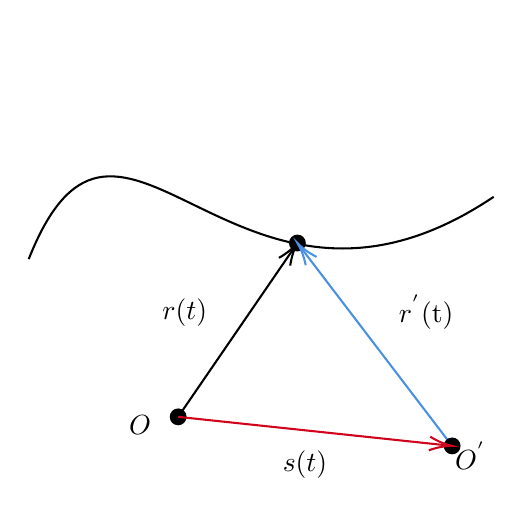
\begin{tikzpicture}[x=0.75pt,y=0.75pt,yscale=-1,xscale=1]
		%uncomment if require: \path (0,402); %set diagram left start at 0, and has height of 402

		%Curve Lines [id:da6494685558841314] 
		\draw    (180.1,126.3) .. controls (224.1,15.3) and (279.1,180.3) .. (404.1,96.3) ;
		%Shape: Circle [id:dp014402697974219558] 
		\draw  [fill={rgb, 255:red, 0; green, 0; blue, 0 }  ,fill opacity=1 ] (306,118.55) .. controls (306,116.59) and (307.59,115) .. (309.55,115) .. controls (311.51,115) and (313.1,116.59) .. (313.1,118.55) .. controls (313.1,120.51) and (311.51,122.1) .. (309.55,122.1) .. controls (307.59,122.1) and (306,120.51) .. (306,118.55) -- cycle ;
		%Straight Lines [id:da09609682920605778] 
		\draw    (252.1,202.3) -- (308.42,120.2) ;
		\draw [shift={(309.55,118.55)}, rotate = 124.45] [color={rgb, 255:red, 0; green, 0; blue, 0 }  ][line width=0.75]    (10.93,-3.29) .. controls (6.95,-1.4) and (3.31,-0.3) .. (0,0) .. controls (3.31,0.3) and (6.95,1.4) .. (10.93,3.29)   ;
		%Shape: Circle [id:dp01339246524637483] 
		\draw  [fill={rgb, 255:red, 0; green, 0; blue, 0 }  ,fill opacity=1 ] (248.55,202.3) .. controls (248.55,200.34) and (250.14,198.75) .. (252.1,198.75) .. controls (254.06,198.75) and (255.65,200.34) .. (255.65,202.3) .. controls (255.65,204.26) and (254.06,205.85) .. (252.1,205.85) .. controls (250.14,205.85) and (248.55,204.26) .. (248.55,202.3) -- cycle ;
		%Straight Lines [id:da544230444191167] 
		\draw [color={rgb, 255:red, 74; green, 144; blue, 226 }  ,draw opacity=1 ]   (384.1,216.3) -- (310.76,120.14) ;
		\draw [shift={(309.55,118.55)}, rotate = 52.67] [color={rgb, 255:red, 74; green, 144; blue, 226 }  ,draw opacity=1 ][line width=0.75]    (10.93,-3.29) .. controls (6.95,-1.4) and (3.31,-0.3) .. (0,0) .. controls (3.31,0.3) and (6.95,1.4) .. (10.93,3.29)   ;
		%Shape: Circle [id:dp8571174104651734] 
		\draw  [fill={rgb, 255:red, 0; green, 0; blue, 0 }  ,fill opacity=1 ] (380.55,216.3) .. controls (380.55,214.34) and (382.14,212.75) .. (384.1,212.75) .. controls (386.06,212.75) and (387.65,214.34) .. (387.65,216.3) .. controls (387.65,218.26) and (386.06,219.85) .. (384.1,219.85) .. controls (382.14,219.85) and (380.55,218.26) .. (380.55,216.3) -- cycle ;
		%Straight Lines [id:da46992008958547604] 
		\draw [color={rgb, 255:red, 208; green, 2; blue, 27 }  ,draw opacity=1 ]   (252.1,202.3) -- (382.11,216.09) ;
		\draw [shift={(384.1,216.3)}, rotate = 186.05] [color={rgb, 255:red, 208; green, 2; blue, 27 }  ,draw opacity=1 ][line width=0.75]    (10.93,-3.29) .. controls (6.95,-1.4) and (3.31,-0.3) .. (0,0) .. controls (3.31,0.3) and (6.95,1.4) .. (10.93,3.29)   ;

		% Text Node
		\draw (227,200) node [anchor=north west][inner sep=0.75pt]   [align=left] {$\displaystyle O$};
		% Text Node
		\draw (384.1,212.75) node [anchor=north west][inner sep=0.75pt]   [align=left] {$\displaystyle O^{'}$};
		% Text Node
		\draw (243,144) node [anchor=north west][inner sep=0.75pt]   [align=left] {$\displaystyle r( t)$};
		% Text Node
		\draw (357,142) node [anchor=north west][inner sep=0.75pt]   [align=left] {$\displaystyle r^{'}$(t)};
		% Text Node
		\draw (301,217) node [anchor=north west][inner sep=0.75pt]   [align=left] {$\displaystyle s( t)$};


	\end{tikzpicture}

\end{mycenter}

Here
\begin{itemize}
	\item The vector $r(t)$ is the position vector of a particle in the inertial frame $O$/relative to $0$.
	\item The vector $r'(t)$ is the position vector of the same particle in the inertial frame $O'$/relative to $O'$.
	\item The vector $s(t)$ represents the shift between the two frames.
\end{itemize}

$$\begin{aligned}\underline{r}(t) = \underline{r^{'}}(t) + \underline{s}(t) & \Rightarrow \underline{\dot{r}}(t) = \underline{\dot{r}}^{'}(t) + \underline{\dot{s}}(t)    \\ \\
                                                                          & \Rightarrow \underline{\ddot{r}}(t) = \underline{\ddot{r}}^{'}(t) + \underline{\ddot{s}}(t)\end{aligned}$$

\clearpage
Since we are working with {\bf inertial frames}, they both must have {\bf constant relative velocity}
$$\underline{s}^{'} = \text{ constant } = \underline{s}^{''}\left(t  \right) = 0$$
i.e. the shift acceleration/relative acceleration is zero.

\begin{definition}[Inertial Frames]
	An {\bf inertial frame} is a frame of reference which is not accelerating and where Newton's law of inertia holds. \\
	If we an inertial frame, {\bf the relative/shift acceleration is 0}
	\begin{equation}
		s^{''}(t) = 0 \tag{$*$} \label{eq: gallilean}
	\end{equation}
	and therefore
	$$\ddot{r}(t) = \ddot{r}^{'}(t)$$

\end{definition}

\subsection{Gallilean Transformation}
We have seen from (\ref{eq: gallilean}) that to have an inertial frame we had
$$\underline{\ddot{s}}\left(t  \right) $$
And then we can solve this differential equation with respect to $t$ to get
$$\underline{\ddot{s}}\left(t  \right) = a + ut$$
where $u$ is a {\bf constant velocity} and $a$ is a {\bf shift in origin}. This is also known as {\bf Gallilean transformation}.

\begin{definition}[Gallilean Transformation]
	A Gallilean Transformation is when the the {\bf shift vector} $s(t)$ is the following:
	\begin{equation}
		\label{eq: gallilean-transformation}
		s(t) = a + ut
	\end{equation}
\end{definition}
